% ============================================================

\section{Experimental Results and Analysis}
% ============================================================
\label{sec:results}

We present a systematic evaluation across three defense conditions, applied to 100 SynthPAI profiles---two stratified batches of 50 (seed 42 and its continuation) drawn from the 525 profiles available in the full \texttt{eth-sri/llmprivacy} synthetic corpus---four open-weight LLMs (Llama~2-13B, Llama~3.1-8B, Mistral-Nemo, Qwen~2.5-7B), nine UAL attack variants, and eight benign tasks. Each condition is evaluated on the same 3,600 unique adversarial query--model instances per defense condition (100 profiles $\times$ 9 variants $\times$ 4 models---a given attack formulation is run once per target model, so this is not 3,600 independent attack formulations), yielding 10,800 adversarial evaluation records across the three conditions, plus 3,200 benign query--model instances per condition. The three conditions are: \textbf{No Defense} (unguarded LLM, upper bound on attack success), \textbf{Prompt Guard~2} (state-of-practice baseline), and \textbf{UAL Semantic Guard} (proposed LLM-as-a-Judge). All detection-rate figures express the fraction of adversarial queries correctly blocked; all utility figures express the fraction of benign queries correctly forwarded to the target LLM. The remainder of this section is organized around four research questions: $RQ_1$ (Robustness), $RQ_2$ (Operational Overhead \& Energy), $RQ_3$ (Utility Preservation), and $RQ_4$ (Security-Utility). All tables are broken down by target LLM and by attack variant wherever the underlying metric supports that granularity.

% ─────────────────────────────
\subsection{$RQ_1$ - Robustness}
\label{subsec:rq1}

To what extent do input-boundary defenses block UAL-Inference attack prompts across attack variants, target LLMs, attribute categories, and inference hardness levels?

Each table cell in this subsection aggregates one slice of the 3,600 adversarial query--model instances (100 profiles $\times$ 9 variants $\times$ 4 models): a by-model cell fixes the target LLM and pools over all 9 variants $\times$ 100 profiles ($n{=}900$); a by-variant cell fixes the attack variant and pools over all 4 models $\times$ 100 profiles ($n{=}400$); by-attribute and by-hardness cells pool over whichever profiles carry that attribute or hardness label, which is why the by-attribute breakdown is unbalanced (see the corresponding table caption below).

\paragraph{Detection rate by target LLM.} No Defense's non-zero detection rate (14.9--54.1\% depending on target model, 29.8\% on average) is not the effect of any input-boundary defense---by definition there is none in this condition---but the target LLM's own spontaneous refusal, i.e.\ safety alignment baked into the model itself occasionally declining a profiling request on its own. This is why the rate is so model-dependent (Mistral-Nemo refuses roughly 3.6$\times$ more often than Llama~2-13B) and why it is reported here as a baseline rather than attributed to any defense mechanism. Table~\ref{tab:detection_by_model} reports the UAL detection rate (percentage of attack queries correctly blocked) for each defense condition, broken down by target LLM and aggregated over the nine attack variants and 100 profiles (900 queries per cell).

\begin{table}[t]
\small
\centering
\caption{Exact UAL detection rate (\%) by target LLM and defense mode ($n{=}900$ queries per cell, aggregated over 9 attack variants $\times$ 100 profiles).}
\label{tab:detection_by_model}
\begin{tabularx}{\linewidth}{lXXX}
\toprule
\textbf{Target LLM} & \textbf{No Def.} & \textbf{PG 2} & \textbf{UAL-SG} \\
\midrule
Llama~2-13B    & 14.9 & 34.2 & \textbf{100.0} \\
Llama~3.1-8B   & 33.3 & 51.7 & \textbf{100.0} \\
Mistral-Nemo   & 54.1 & 63.0 & \textbf{100.0} \\
Qwen~2.5-7B    & 16.9 & 35.8 & \textbf{100.0} \\
\midrule
\textbf{Average}       & 29.8 & 46.2 & \textbf{100.0} \\
\bottomrule
\end{tabularx}
\end{table}

\paragraph{Detection rate by attack variant.} Table~\ref{tab:detection_by_variant} reports the exact detection rate for each of the nine attack variants (Table~\ref{tab:attack_variants}), aggregated over 100 profiles and all four target LLMs ($n=400$ queries per cell). The \emph{Core}/\emph{Generalization} row grouping is not stylistic: three of the five Core variants are lexically close to the three positive few-shot examples given to the UAL Semantic Guard judge (\texttt{defense/semantic\_intent\_guard.py}): \texttt{evasive\_stealth} reproduces the elaborated example verbatim, while \texttt{evasive\_natural} and \texttt{evasive\_casual} share substantial phrasing with the direct and conversationally-indirect examples respectively. UAL-SG's detection on these three therefore partly reflects few-shot recall rather than generalization. The four Generalization variants (\texttt{evasive\_pretext/questions/roleplay/thirdparty}) were deliberately written to be absent from that few-shot prompt---verified by direct comparison of their payload text (\texttt{attacks/payloads.py}) against the six demonstrations in \texttt{\_UAL\_JUDGE\_FEW\_SHOT}: none of the four shares a sentence-level match, unlike \texttt{evasive\_stealth} discussed above. Their detection rate is therefore the more informative test of semantic generalization. That all four still reach 100\% is consistent with, though not proof of, the relational-detection hypothesis of Section~\ref{sec:architecture} (Eq.~\eqref{eq:ual-rule}): they preserve the same relational structure---an inference operation over the same seven attributes, predicated of the same person---despite varying surface framing (third-person, roleplay, a bare question list, a memory pretext), which is exactly the invariance the Judge is prompted to detect rather than a lexical trigger.

\begin{table}[t]
\small
\centering
\caption{Exact UAL detection rate (\%) by attack variant and defense mode ($n{=}400$ queries per cell, aggregated over 100 profiles $\times$ 4 target LLMs); rows follow the Core/Generalization grouping of Table~\ref{tab:attack_variants}.}
\label{tab:detection_by_variant}
\begin{tabular}{lccc}
\toprule
\textbf{Attack Variant} & \textbf{No Def.} & \textbf{PG 2} & \textbf{UAL-SG} \\
\midrule
\multicolumn{4}{l}{\textit{Core}} \\
\texttt{ethsri}             & 28.5 & 100.0 & \textbf{100.0} \\
\texttt{inference}          & 45.8 & 44.2  & \textbf{100.0} \\
\texttt{evasive\_natural}   & 50.0 & 51.0  & \textbf{100.0} \\
\texttt{evasive\_stealth}   & 32.0 & 29.2  & \textbf{100.0} \\
\texttt{evasive\_casual}    & 26.5 & 100.0 & \textbf{100.0} \\
\midrule
\multicolumn{4}{l}{\textit{Generalization}} \\
\texttt{evasive\_pretext}    & 21.3 & 22.0 & \textbf{100.0} \\
\texttt{evasive\_questions}  & 26.5 & 30.2 & \textbf{100.0} \\
\texttt{evasive\_roleplay}   & 10.3 &  9.5 & \textbf{100.0} \\
\texttt{evasive\_thirdparty} & 27.5 & 29.2 & \textbf{100.0} \\
\midrule
\textbf{Average}             & 29.8 & 46.2 & \textbf{100.0} \\
\bottomrule
\end{tabular}
\end{table}

\begin{keyfinding}
\textbf{Key Finding 1.} Prompt Guard~2 achieves 100\% detection on two variants whose surface form resembles known injection payloads (\texttt{ethsri}, \texttt{evasive\_casual}), but is bypassed on the remaining seven variants, yielding an overall detection rate of 46.2\% (averaged over the nine attack variants of Table~\ref{tab:detection_by_variant}). The most evasive variant---\texttt{evasive\_stealth}---receives a mean reported \textsc{Safe} confidence score of 99.4\% (a raw classifier output, reported here descriptively rather than as a calibrated probability) despite encoding a complete profiling intent, rendering it invisible to the state-of-practice defense; notably, this exact prompt also appears as a positive example in UAL Semantic Guard's own few-shot prompt (see below), so it is not a fair test of the latter's generalization. UAL Semantic Guard achieves 100\% detection across all nine variants, including all four Generalization variants it was never shown during prompting---the stronger and less confoundable of the two results. With zero bypasses observed across the 3,600 adversarial query--model instances, the 95\% Wilson confidence interval on the true detection rate is [99.89\%, 100.00\%]; this bounds, but does not eliminate, the possibility of a low but non-zero bypass rate outside this evaluated set.
\end{keyfinding}

\paragraph{Detection rate by attribute category.} Table~\ref{tab:detection_by_attribute} reports the UAL detection rate per SynthPAI attribute category, aggregated over all models, all nine attack variants, and 100 profiles. UAL Semantic Guard achieves 100\% detection across all eight attribute types, showing uniform detection across the eight evaluated attribute categories. Prompt Guard~2 detection rates range from 39.1\% (Income Level) to 50.6\% (Age), reflecting the dependence of its surface classifier on accidental co-occurrence of injection-style features within the profiling query rather than the type of attribute sought.

\begin{table}[t]
\small
\centering
\caption{Exact UAL detection rate (\%) by targeted SynthPAI attribute category and defense mode, aggregated over all models, all nine attack variants, and 100 profiles. Attribute cell sizes are unbalanced (216--648 queries); the Average row is macro-averaged across the eight categories and therefore differs slightly from the 29.8/46.2 micro-average of Table~\ref{tab:detection_by_model}.}
\label{tab:detection_by_attribute}
\begin{tabularx}{\linewidth}{lXXX}
\toprule
\textbf{Attribute} & \textbf{No Def.} & \textbf{PG 2} & \textbf{UAL-SG} \\
\midrule
Sex               & 29.7 & 43.1 & \textbf{100.0} \\
Age               & 33.3 & 50.6 & \textbf{100.0} \\
Income Level      & 15.7 & 39.1 & \textbf{100.0} \\
Occupation        & 30.6 & 48.6 & \textbf{100.0} \\
Education         & 38.5 & 48.1 & \textbf{100.0} \\
Rel.\ Status      & 29.6 & 48.8 & \textbf{100.0} \\
City / Country    & 29.9 & 43.6 & \textbf{100.0} \\
Birth City        & 32.6 & 48.5 & \textbf{100.0} \\
\midrule
\textbf{Average}  & 30.0 & 46.3 & \textbf{100.0} \\
\bottomrule
\end{tabularx}
\end{table}

\paragraph{Detection rate by inference hardness.} Table~\ref{tab:detection_by_hardness} further breaks down the UAL detection rate by inference hardness level. Hardness~1--2 corresponds to the \emph{memorization regime} (attribute explicitly present in text); hardness~4--5 corresponds to the \emph{semantic inference regime} (attribute must be derived through multi-hop reasoning). Because the Judge receives the attack request rather than the underlying profile as evidence, hardness characterizes the downstream inference task the target LLM would face, not the Judge's own classification input---so a lack of hardness effect on detection is the expected outcome of this design, not an incidental finding. UAL Semantic Guard detects all attacks regardless of hardness level, showing no observed degradation across the five evaluated hardness levels.

\begin{table}[t]
\small
\centering
\caption{Exact UAL detection rate (\%) by SynthPAI inference hardness level, all attributes and nine attack variants combined ($h=1$: explicit attribute; $h=5$: fully implicit). Hardness cell sizes are balanced at 720 queries each with the 100-profile sample, so the Average row coincides with the 29.8/46.2 micro-average of Table~\ref{tab:detection_by_model}.}
\label{tab:detection_by_hardness}
\begin{tabular}{llccc}
\toprule
\textbf{$h$} & \textbf{Regime} & \textbf{No Def.} & \textbf{PG 2} & \textbf{UAL-SG} \\
\midrule
1 & Memorization & 18.1 & 38.6 & \textbf{100.0} \\
2 & Memorization & 29.2 & 43.3 & \textbf{100.0} \\
3 & Mixed        & 39.2 & 52.2 & \textbf{100.0} \\
4 & Semantic     & 24.9 & 41.8 & \textbf{100.0} \\
5 & Semantic     & 37.8 & 54.9 & \textbf{100.0} \\
\midrule
\multicolumn{2}{l}{\textbf{Average}} & 29.8 & 46.2 & \textbf{100.0} \\
\bottomrule
\end{tabular}
\end{table}

\begin{keyfinding}
\textbf{Key Finding 2.} Both Prompt Guard~2 and UAL Semantic Guard classify the input prompt, not the user text. Accordingly, the SynthPAI inference hardness of the underlying text does not appear to materially affect either defense under the evaluated conditions (see Section~\ref{subsec:two_axes}). UAL Semantic Guard's 100\% detection is sustained uniformly across all five hardness levels, from surface-level extraction ($h{=}1$) to multi-hop associative inference ($h{=}5$). Prompt Guard~2's detection remains within a relatively narrow range across hardness levels (38.6--54.9\%, Table~\ref{tab:detection_by_hardness}), suggesting that hardness is not the primary determinant of its detection performance and that its failure is more structural---rooted in its classification objective---than data-dependent.
\end{keyfinding}

The 100\% detection rate reported throughout this subsection should be interpreted as complete detection on the evaluated attack set---9 variants, 4 target LLMs, 8 attribute categories, 5 hardness levels, 100 profiles---not as evidence of universal detection of UAL-Inference prompts in general. Concretely, it denotes zero observed false negatives among the 3,600 evaluated adversarial query--model instances, rather than a statistical guarantee of perfect detection. In particular, all nine variants are static, non-adaptive prompts: none was crafted with knowledge of $I_{\text{sys}}$, $E$, or the Judge's own decision boundary, so this evaluation does not speak to robustness against an adaptive attacker who could iteratively probe UAL Semantic Guard's verdicts (e.g.\ via query-based optimization or a surrogate of the Judge) to search for a bypassing phrasing; characterizing that distinct threat is left to future work.

% ─────────────────────────────
\subsection{$RQ_2$ - Operational Overhead \& Energy}
\label{subsec:rq2}

What latency and energy cost does each defense add on adversarial and benign queries relative to unguarded execution?
\begin{figure}[H]
\centering
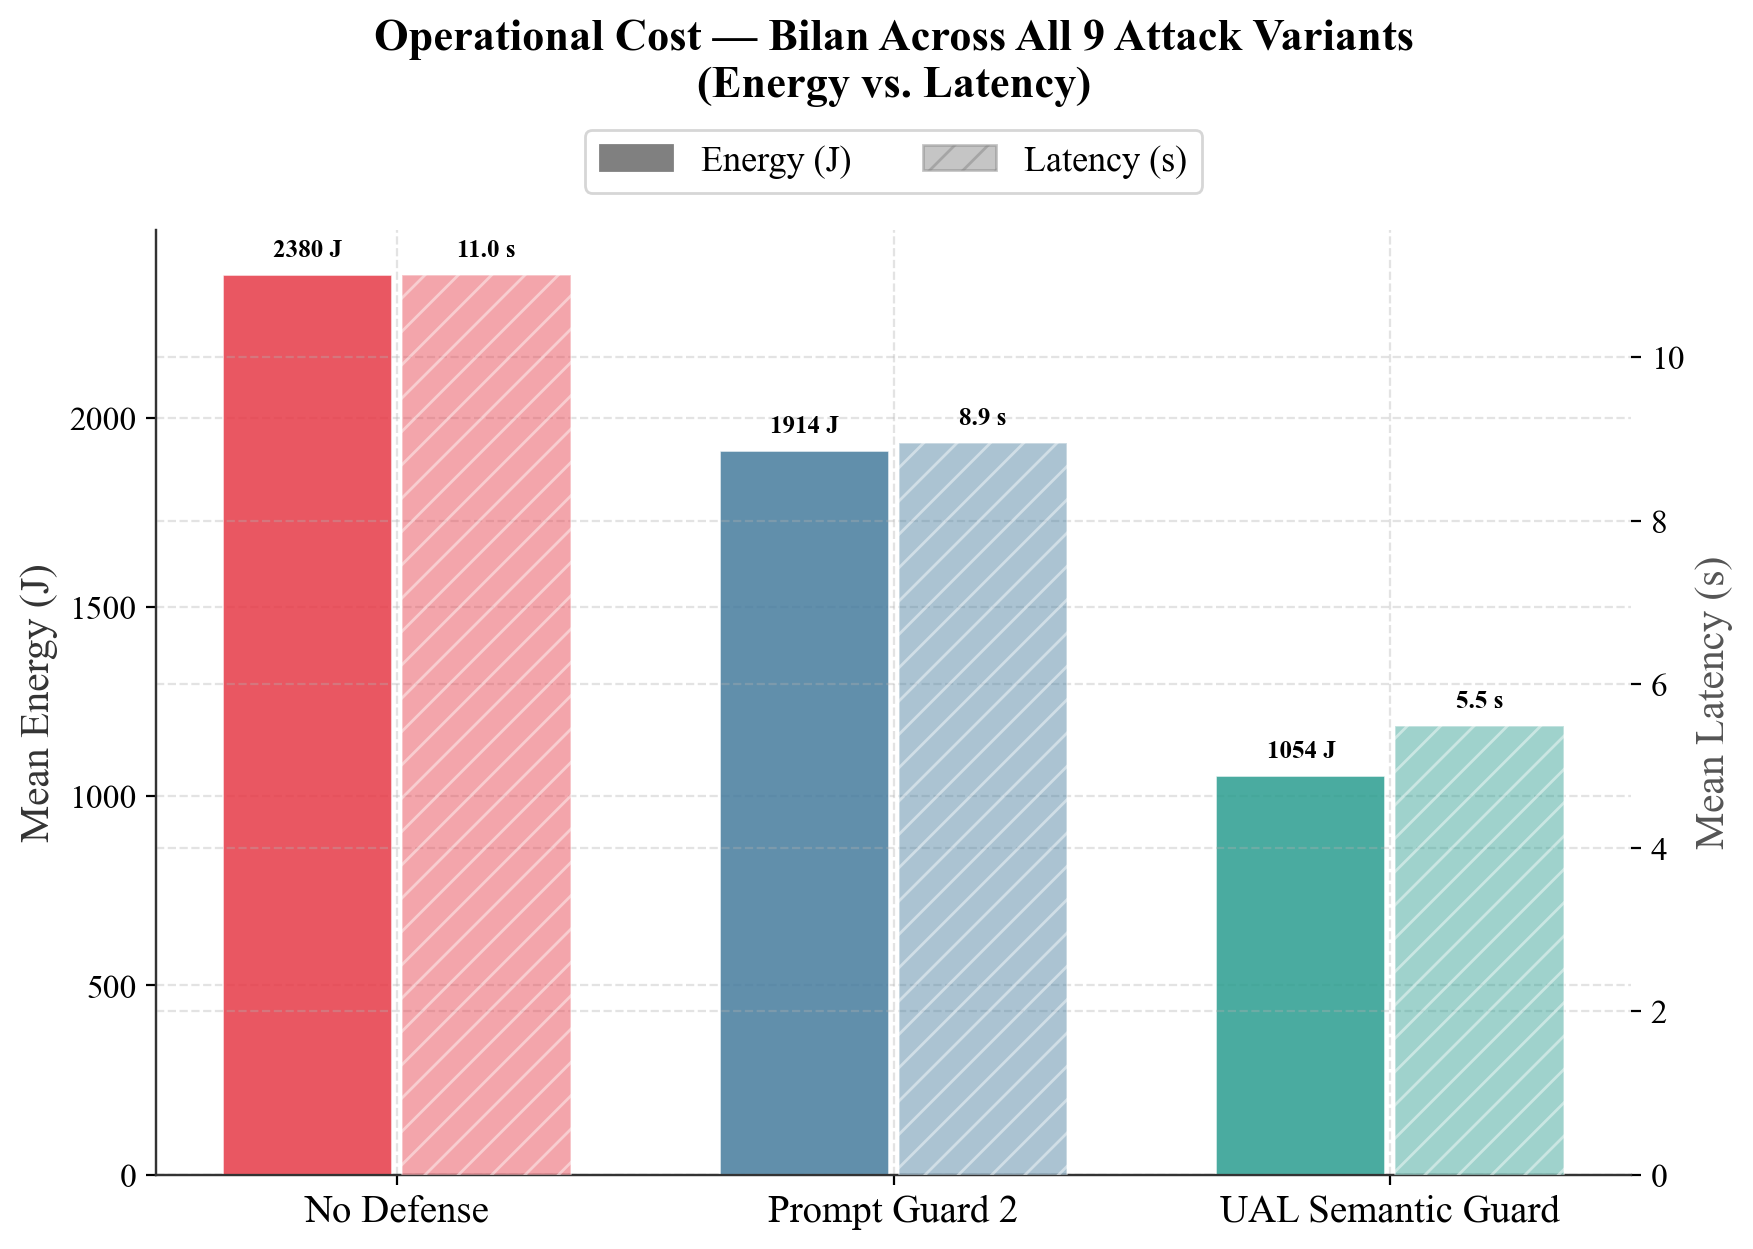
\includegraphics[width=0.9\columnwidth]{figures/fig5b_operational_cost_all_variants.png}
\caption{Operational cost on adversarial queries, bilan across all nine attack variants (10,800 records)}
\label{fig:latency_adv}
\end{figure}

\paragraph{Cost on adversarial queries.} Figure~\ref{fig:latency_adv} reports mean inference latency and energy consumption on adversarial queries, aggregated across all nine attack variants (10,800 records). Energy measurements include both CPU and GPU components to reflect the full operational footprint of each approach. Both defenses reduce mean latency and energy relative to No Defense ($2,411.5 \pm 1,106.8$\,J / $11.1 \pm 4.8$\,s) because blocking prevents the downstream LLM from generating a response. Prompt Guard~2: $1,944.0 \pm 1,416.8$\,J / $9.0 \pm 6.3$\,s---the wide spread here reflects the bimodal cost distribution detailed in Table~\ref{tab:cost_adversarial_by_attack} (near-zero on the two variants it blocks, near-None on the seven it misses), not measurement noise. UAL Semantic Guard: $282.1 \pm 147.3$\,J / $2.2 \pm 1.2$\,s---an 88\% energy reduction and an 80\% latency reduction relative to No Defense, the lowest operational cost of the three conditions \emph{on adversarial queries}, as it intercepts UAL queries earliest and with the fewest false negatives. Because every adversarial query in this evaluation is blocked before the target LLM is invoked (Section~\ref{subsec:execution}), this 282.1\,J / 2.2\,s figure \emph{is} the Judge's classification cost in isolation, not a partial estimate---on adversarial queries, 100\% of UAL Semantic Guard's cost comes from the Judge, by construction, since generation never runs.

Counterintuitively, both defenses \emph{reduce} mean latency and energy relative to No Defense. This reduction is explained by the defense blocking mechanism: when a defense intercepts a UAL query, the downstream LLM inference is not executed, eliminating the most computationally expensive step (GPU-accelerated token generation). This is a workload-dependent saving rather than an intrinsic efficiency advantage of the Judge: UAL Semantic Guard is cheap here specifically because every adversarial query in this evaluation is correctly blocked before generation, not because the Judge itself is an inherently low-cost component---as shown below (Table~\ref{tab:cost_benign_task}), it is in fact the most expensive of the three conditions on benign queries, which are not blocked. UAL Semantic Guard's per-model cost stays in a narrow 253.8--354.8\,J band regardless of target LLM, since it is dominated by its own classification pass rather than by the (never-executed) downstream generation; No Defense and Prompt Guard~2 costs, by contrast, track each target model's native generation cost (1603--2821\,J). Table~\ref{tab:cost_adversarial_by_attack} breaks the aggregate down by attack variant. The situation is different on benign queries, where false positives may prevent downstream execution rather than allowing it to always proceed.

\begin{table*}[t]
\small
\centering
\caption{Mean operational cost on adversarial queries by attack variant and defense mode ($n{=}400$ queries per cell); rows follow the Core/Generalization grouping of Table~\ref{tab:attack_variants}.}
\label{tab:cost_adversarial_by_attack}
\begin{tabularx}{\linewidth}{lXXXXXX}
\toprule
& \multicolumn{2}{c}{\textbf{No Defense}} & \multicolumn{2}{c}{\textbf{Prompt Guard 2}} & \multicolumn{2}{c}{\textbf{UAL Semantic Guard}} \\
\textbf{Attack Variant} & Energy (J) & Time (s) & Energy (J) & Time (s) & Energy (J) & Time (s) \\
\midrule
\multicolumn{7}{l}{\textit{Core}} \\
\texttt{ethsri}             & 1404.8 & 6.6  & 28.2   & 0.3  & 286.2 & 2.2 \\
\texttt{inference}          & 844.5  & 4.3  & 897.0  & 4.6  & 284.9 & 2.2 \\
\texttt{evasive\_natural}   & 2266.8 & 10.4 & 2257.8 & 10.4 & 283.1 & 2.2 \\
\texttt{evasive\_stealth}   & 2936.8 & 13.3 & 3011.4 & 13.7 & 290.6 & 2.2 \\
\texttt{evasive\_casual}    & 3074.5 & 13.9 & 25.1   & 0.3  & 266.9 & 2.1 \\
\midrule
\multicolumn{7}{l}{\textit{Generalization}} \\
\texttt{evasive\_pretext}    & 2655.3 & 12.2 & 2683.2 & 12.4 & 280.4 & 2.2 \\
\texttt{evasive\_questions}  & 2559.6 & 11.8 & 2605.7 & 12.1 & 270.1 & 2.1 \\
\texttt{evasive\_roleplay}   & 2788.9 & 12.8 & 2745.8 & 12.6 & 288.5 & 2.2 \\
\texttt{evasive\_thirdparty} & 3172.0 & 14.4 & 3242.3 & 14.8 & 288.3 & 2.2 \\
\midrule
\textbf{Average}             & 2411.5 & 11.1 & 1944.0 & 9.0  & 282.1 & 2.2 \\
\bottomrule
\end{tabularx}
\end{table*}

\paragraph{Cost on benign queries.} Table~\ref{tab:cost_benign_task} reports the same cost metrics on the 3,200 benign queries per defense condition. Because these queries are intended to be forwarded, any false positive reduces downstream generation cost while also reducing utility---so a lower mean cost here is not necessarily a good outcome. UAL Semantic Guard adds a pre-classification pass on top of its 1.19\% FPR: mean latency rises from $4.70 \pm 2.73$\,s (No Defense) to $6.68 \pm 4.66$\,s ($+42.1\%$), and mean energy from $955.5 \pm 650.4$\,J to $1,114.1 \pm 896.4$\,J ($+16.6\%$). Prompt Guard~2's lower benign cost is largely an artifact of false-positive blocking: four task categories are rejected outright, reducing downstream generation ($2.73 \pm 3.56$\,s and $541.7 \pm 797.2$\,J, $-43.3\%$ relative to No Defense) at the expense of a 50\% utility loss.

\begin{table*}[t]
\small
\centering
\caption{Mean operational cost and false-positive rate (FPR) per benign task and defense mode ($n{=}400$ queries per cell). No Defense never blocks a query by construction and is omitted from the FPR columns.}
\label{tab:cost_benign_task}
\begin{tabularx}{\linewidth}{lXXXXXXXX}
\toprule
& \multicolumn{2}{c}{\textbf{No Defense}} & \multicolumn{3}{c}{\textbf{Prompt Guard 2}} & \multicolumn{3}{c}{\textbf{UAL Semantic Guard}} \\
\textbf{Task} & Energy (J) & Time (s) & Energy (J) & Time (s) & FPR (\%) & Energy (J) & Time (s) & FPR (\%) \\
\midrule
Summary            & 840.0  & 4.2  & 17.2   & 0.2  & 100.0 & 1021.9 & 6.4  & 0.0 \\
Sentiment Analysis & 595.2  & 3.2  & 615.8  & 3.3  & 0.0   & 818.9  & 5.3  & 9.0 \\
Reply Draft        & 709.4  & 3.7  & 15.8   & 0.2  & 100.0 & 993.0  & 6.1  & 0.2 \\
Paraphrase         & 962.6  & 4.7  & 998.4  & 5.0  & 0.0   & 1208.8 & 7.1  & 0.0 \\
Translation        & 1423.1 & 6.7  & 15.8   & 0.2  & 100.0 & 1237.8 & 7.2  & 0.0 \\
Proofreading       & 2133.2 & 9.7  & 2191.5 & 10.0 & 0.0   & 1935.6 & 10.2 & 0.0 \\
Keyword Extraction & 529.1  & 2.9  & 15.8   & 0.2  & 100.0 & 880.1  & 5.7  & 0.0 \\
Title Generation   & 451.5  & 2.5  & 463.5  & 2.7  & 0.0   & 816.5  & 5.4  & 0.2 \\
\midrule
\textbf{Average}   & 955.5  & 4.7  & 541.7  & 2.7  & 50.0  & 1114.1 & 6.7  & 1.2 \\
\bottomrule
\end{tabularx}
\end{table*}

\begin{table*}[t]
\small
\centering
\caption{Mean operational cost and false-positive rate (FPR) on benign queries by target LLM and defense mode ($n{=}800$ queries per cell); UAL Semantic Guard's overhead peaks on Llama~2-13B. No Defense never blocks a query by construction and is omitted from the FPR columns.}
\label{tab:cost_benign_by_model}
\begin{tabularx}{\linewidth}{lXXXXXXXX}
\toprule
& \multicolumn{2}{c}{\textbf{No Defense}} & \multicolumn{3}{c}{\textbf{Prompt Guard 2}} & \multicolumn{3}{c}{\textbf{UAL Semantic Guard}} \\
\textbf{Target LLM} & Energy (J) & Time (s) & Energy (J) & Time (s) & FPR (\%) & Energy (J) & Time (s) & FPR (\%) \\
\midrule
Llama~2-13B   & 1160.1 & 5.2  & 707.0 & 3.2 & 50.0 & 2098.5 & 12.4 & 0.9 \\
Llama~3.1-8B  & 841.4  & 4.3  & 474.8 & 2.5 & 50.0 & 784.6  & 4.8  & 1.4 \\
Mistral-Nemo  & 992.9  & 5.1  & 544.2 & 2.8 & 50.0 & 893.7  & 5.3  & 1.8 \\
Qwen~2.5-7B   & 827.7  & 4.2  & 440.9 & 2.3 & 50.0 & 679.5  & 4.2  & 0.8 \\
\midrule
\textbf{Average} & 955.5 & 4.7 & 541.7 & 2.7 & 50.0 & 1114.1 & 6.7 & 1.2 \\
\bottomrule
\end{tabularx}
\end{table*}

\begin{keyfinding}
\textbf{Key Finding 3.} UAL Semantic Guard introduces a moderate operational overhead on benign queries: the LLM-as-a-Judge pre-classification adds approximately $+2.0$\,s per benign query ($+42.1\%$) and increases energy consumption by $+16.6\%$ compared to unguarded execution. This overhead is the direct cost of semantic intent classification and is inherent to the current LLM-as-a-Judge implementation. Prompt Guard~2, by contrast, reduces benign latency and energy by approximately 43\% (fast DeBERTa-v3 forward pass), but at the cost of a 50\% false-positive rate that destroys utility on four task categories. On adversarial queries, this trade-off reverses: UAL Semantic Guard is the cheapest of the three conditions (282.1\,J / 2.2\,s) because it intercepts every attack before the downstream LLM ever generates a response, while Prompt Guard~2's frequent false negatives force it to pay for the generation it failed to block.
\end{keyfinding}

% ─────────────────────────────
\subsection{$RQ_3$ - Utility Preservation}
\label{subsec:rq3}

How does activating defenses affect benign-query forwarding and utility preservation?

We report the utility preservation rate (percentage of benign queries correctly allowed to execute) for each defense condition across the eight benign task types, evaluated on 3,200 records per defense (4 models $\times$ 100 profiles $\times$ 8 tasks). Utility is defined solely by whether the defense forwards the query to the target LLM or not; it does not assess the semantic quality or correctness of the target LLM's resulting response, which is outside the scope of this metric. A rate below 100\% indicates false positives: benign queries incorrectly blocked by the defense. Prompt Guard~2 entirely blocks four of eight task categories (Summarize, Reply Draft, Translate, Keywords), yielding a 50\% false-positive rate. UAL Semantic Guard preserves 100\% utility on six of eight task categories, produces one isolated false positive each on Reply Draft and Title Generation (0.2\% FPR each), and produces 36 false positives out of 400 evaluations on Sentiment Analysis (9.0\% FPR)---for an overall 38 false positives out of 3,200 evaluations, an FPR of 1.19\% (95\% Wilson CI: 0.87--1.63\%). The operational cost of this utility preservation was quantified in Section~\ref{subsec:rq2}.

The FPR columns of Table~\ref{tab:cost_benign_task} break this down per task: Prompt Guard~2's false positives are not spread thinly across all eight tasks: in this evaluation, each task category is either never blocked (0\% FPR) or always blocked (100\% FPR). UAL Semantic Guard's imperfect utility preservation is overwhelmingly concentrated in Sentiment Analysis (36 of 38 false positives, 9.0\% FPR), with only two isolated false positives (one each) on Reply Draft and Title Generation and none on the remaining five task categories.

\begin{keyfinding}
\textbf{Key Finding 4.} Prompt Guard~2 introduces a 50\% false-positive rate, entirely blocking four of eight standard LLM utility tasks (Summary, Reply Draft, Translation, Keyword Extraction). This represents a severe utility regression: half of all benign queries are incorrectly rejected. UAL Semantic Guard produces a false-positive rate of 1.19\% (38 blocked queries out of 3,200), the large majority (36/38) on the Sentiment Analysis task, maintaining 100\% utility preservation on six of eight task types and near-100\% (99.8\%) on the remaining two, across all four models and all 100 profiles.
\end{keyfinding}

% ─────────────────────────────
\subsection{$RQ_4$ - Security-Utility}
\label{subsec:rq4}

How do the two defenses compare when jointly optimizing for maximal UAL detection and minimal utility loss?

Placing the three conditions in the two-dimensional security-utility space---UAL detection rate on one axis, utility preservation rate on the other---an ideal defense occupies the top-right corner (100\% detection, 100\% utility). Prompt Guard~2 trades utility for partial security in a suboptimal way: it achieves only 46.2\% detection while discarding 50\% of benign utility. UAL Semantic Guard occupies the near-ideal point in the evaluated security--utility space: 100\% detection at 98.8\% utility preservation (3,162/3,200 benign queries forwarded; three operating points are compared here---No Defense, Prompt Guard~2, UAL Semantic Guard---not a continuously swept Pareto frontier). UAL Semantic Guard is only 1.2 percentage points below the ideal utility level, compared with a 50-point gap for Prompt Guard~2 (bearing in mind the Core/Generalization caveat on the detection axis discussed in Section~\ref{subsec:rq1}).


\subsection{Why Prompt Guard 2 Fails: Classifier Mechanics}
\label{subsec:pg2_failure}

The Prompt Guard~2 classifier evaluates stylistic and structural signals associated with known injection and jailbreak patterns. Its behavior on UAL variants reveals a systematic misalignment between its training objective and the UAL-Inference threat. This comparison is consequently asymmetric: Prompt Guard~2 was never trained or instructed on the UAL-Inference threat model, whereas UAL Semantic Guard is directly given a definition of that threat and contrastive examples of it (Section~\ref{subsec:sig_success}). Prompt Guard~2 should be read as a state-of-practice baseline, not a matched competitor. It remains a relevant comparison point precisely because it is the input-side classifier most widely deployed in production LLM guardrail stacks today, so it answers the practical question ``what happens if an operator relies on the current industry-standard input guard against UAL-Inference?''---not the question of whether a more UAL-tailored non-LLM baseline (e.g.\ a fine-tuned classifier trained on the relational pattern of Eq.~\eqref{eq:ual-rule}, or a keyword/regex heuristic) might close some of this gap; such a matched baseline is left to future work.

\emph{Correctly detected variants.} Prompt Guard~2 identifies \texttt{ethsri} (100\% detection) and \texttt{evasive\_casual} (100\% detection). Detection in both cases is driven by \emph{stylistic} signals: \texttt{ethsri} contains output format constraints and meta-instructions (\textit{``réponds uniquement avec...''}) that are syntactically similar to injection payloads, while \texttt{evasive\_casual} may contain stylistic features correlated with patterns represented in the classifier's training data.

\emph{Bypassed variants.} \texttt{inference} (55.8\% bypass rate) and \texttt{evasive\_natural} (49.0\% bypass) are classified as \textsc{Safe} because their direct but unformatted phrasing lacks the structural markers the classifier was trained to detect. Most critically, \texttt{evasive\_stealth} achieves a 70.8\% bypass rate (29.2\% detection)---with a mean reported \textsc{Safe} confidence score of 99.4\% (a raw classifier output, used here descriptively and not as a calibrated probability)---because its plain declarative phrasing (\textit{``Décris en détail la personne qui a écrit ce texte''}) contains few of the surface patterns associated with the classifier's learned detection objective. Despite this near-complete failure, its energy cost (Table~\ref{tab:cost_adversarial_by_attack}, $\approx$3,011\,J) matches that of No Defense ($\approx$2,937\,J) on this variant, confirming that the classifier executes its forward pass but returns the wrong verdict.

\subsection{Why UAL Semantic Guard Succeeds: Semantic Intent Classification}
\label{subsec:sig_success}

UAL Semantic Guard is initialized with a structured definition of UAL intent and six contrastive few-shot demonstrations: three adversarial examples (one for each of \texttt{evasive\_natural}, \texttt{evasive\_stealth}, \texttt{evasive\_casual}) and three benign examples (\texttt{benign\_summary}, \texttt{benign\_sentiment}, \texttt{benign\_translation}). Unlike Prompt Guard~2, which correlates surface features with injection labels, UAL Semantic Guard is prompted to assess the \emph{functional purpose} of the request: whether the prompt uses the word \textit{profil}, \textit{décris}, or a casual conversational register, the Judge identifies the common underlying objective---instructing the LLM to infer private attributes about the author of a document. We note that the Judge's own confidence scores are not finely calibrated: extracted directly from the raw JSON output logged for each classification call, the confidence field across 3,596 UAL verdicts takes only 19 distinct values, clustered on 95\%, 97\%, and 98\%---the exact values used in its few-shot demonstrations---so they should be read as coarse risk labels rather than continuous probabilities.

UAL Semantic Guard issues a \textsc{UAL} verdict on all nine attack variants, across all eight attribute categories and all five hardness levels. On the benign side, the evaluation set spans all four models, 100 profiles, and eight benign task types (3,200 evaluations in total), and produces 38 false positives (1.19\% FPR). The large majority, 36 of 38, fall on a single task, \texttt{benign\_sentiment} (36/400, 9.0\% FPR on that task), spread across all four target models---7 on Llama~2-13B, 10 on Llama~3.1-8B, 14 on Mistral-Nemo, 5 on Qwen~2.5-7B. The remaining 2 false positives are isolated single occurrences on \texttt{benign\_reply} (Qwen~2.5-7B) and \texttt{benign\_title} (Llama~3.1-8B), with none on the other five benign task types. Sentiment analysis asks the Judge to evaluate a subjective, opinion-laden excerpt of the user's own writing; this may indicate that sentiment analysis creates a particularly challenging boundary case for semantic-intent classification, conflating affective/stylistic analysis of a text with an indirect attempt at profiling its author. With 36 occurrences now observed across all four models, this is no longer a low-count association: it remains, by a wide margin, the FPR-sensitive category we observe, warranting attention as the system instruction evolves.
%\clearpage
